\subsection{Quantile Autoregression with a nonparametric approach}
\label{sec:npqar}

Fitting a linear estimator for the Quantile Auto Regression isn't appropriate  when nonlinearity is present in the data. This nonlinearity may produce a linear estimator that underestimates the quantile for a chunk of data while overestimating for the other chunk. To prevent this issue from occurring we propose a modification which we let the prediction $q_\alpha(x_t)$ adjust freely to the data and its nonlinearities. To prevent overfitting and smoothen our predictor, we include a penalty on its roughness by including the $\ell_1$ norm of its second derivative. For more information on the $\ell_1$ norm acting as a filter, one can refer to \cite{kim2009ell_1}.

This time, as opposed to when employing linear models, we don't suppose any functional form for $q_\alpha(x_t)$. This forces us to build each $q_\alpha$ differently: instead of finding a set of parameters that fully defines the function, we find a value for $q_\alpha(x_t)$ at each instant $t$. On the optimization problem, we will find optimal values for a variable $q_{\alpha t} \in \mathbb{R}$, each consisting of a single point. The sequence  $\{ q^*_{\alpha t} \}_{\alpha \in A} $ will provide a discretization for the quantile function $\hat{q}_\alpha(x_t)$, which can be found by interpolating these points.

% notação estatística de ordem. com x^(0)

Let $\{\tilde{y}_t \}_{t=1}^n$ be the sequence of observations in time $t$. Now, let $\tilde{x}_t$ be the $p-$lagged time series of $\tilde{y}_t$, such that $\tilde{x}_t = L^p(\tilde{y}_t)$, where $L$ is the lag operator. Matching each observation $\tilde{y}_t$ with its $p-$lagged correspondent $\tilde{x}_t$ will produce $n-p$ pairs $\{(\tilde{y}_t,\tilde{x}_t)\}_{t=p+1}^n$ (note that the first $p$ observations of $y_t$ must be discarded). When we order the observation of $x$ in such way that they are in growing order
$$\tilde{x}^{(p+1)} \leq \tilde{x}^{(p+2)} \leq \dots \leq \tilde{x}^{(n)},$$ 
we can then define $\{x_i\}_{i=1}^{n-p} = \{\tilde{x}^{(t)} \}_{t=p+1}^{n}$ and $\{y_i\}_{i=1}^{n-p} = \{\tilde{y}^{(t)} \}_{t=p+1}^{n}$ and $T' = \{2,\dots, n-p-1\}$. 

Our optimization model to estimate the nonparametric quantile is as follows:
\begin{equation}
\begin{split}
\hat{q}_\alpha(x_t) =\underset{q_{\alpha t}}{\arg\min}\sum_{t\in T'} \left( \alpha |y_{t}-q_{\alpha t}|^{+} + (1-\alpha)|y_{t}-q_{\alpha t}|^{-}\right) \\ +\lambda_1  \sum_{t\in T'}|D_{x_t}^{1}q_{\alpha t}| +\lambda_2  \sum_{t\in T'}|D_{x_t}^{2}q_{\alpha t}|,
\end{split}
\end{equation}
where $D^1 q_t$ and $D^2 q_t$ are the first and second derivatives of the $q_\alpha(x_t)$ function, calculated as follows:
\begin{equation*}
D_{x_{t}}^{2}q_{\alpha t}=\frac{\left(\frac{q_{\alpha t+1}-q_{\alpha t}}{x_{t+1}-x_{t}}\right)-\left(\frac{q_{\alpha t}-q_{\alpha t-1}}{x_{t}-x_{t-1}}\right)}{x_{t+1}-2x_{t} + x_{t-1}},
\end{equation*}


\begin{equation*}
D^{1}_{t \alpha }=\frac{q_{\alpha t+1}-q_{\alpha t}}{x_{t+1}-x_{t}}.
\end{equation*}
The first part on the objective function is the usual quantile regression condition for $\{q_{t\alpha}\}_{\alpha \in A}$. The second part is the $\ell_1$-filter. The purpose of a filter is to control the amount of variation for our estimator $q_\alpha(x_t)$. When no penalty is employed we would always get $q_{\alpha t} = y_t$, for any given $\alpha$. On the other hand, when $\lambda_2 \rightarrow \infty$, our estimator approaches the linear quantile regression. 

The full model can be rewritten as a LP problem as bellow:
\begin{eqnarray}
\min_{q_{\alpha t},\delta^+_{t}, \delta_t^-, \xi_t} & \sum_{\alpha \in A} \sum_{t \in T'}\left(\alpha\delta_{t \alpha }^{+}+(1-\alpha)\delta_{t \alpha }^{-}\right) & \\
& \qquad \qquad \qquad \qquad \qquad + \lambda_1\sum_{t \in T'}\gamma_{t \alpha } + \lambda_2\sum_{t \in T'}\xi_{t \alpha } & \nonumber \\
s.t. & \delta_{t}^{+}-\delta_{t \alpha }^{-}=y_{t}-q_{t \alpha }, & \qquad\forall t \in T',\forall \alpha \in A,\\
   & D^{1}_{t \alpha }=\frac{q_{\alpha t+1}-q_{\alpha t}}{x_{t+1}-x_{t}},
    & \qquad\forall t \in T',\forall \alpha \in A,\\   
 & D^{2}_{t \alpha }=\frac{\left(\frac{q_{\alpha t+1}-q_{\alpha t}}{x_{t+1}-x_{t}}\right)-\left(\frac{q_{\alpha t}-q_{\alpha t-1}}{x_{t}-x_{t-1}}\right)}{x_{t+1}-2x_{t} + x_{t-1}}.
  & \qquad\forall t \in T',\forall \alpha \in A,\\
 & \gamma_{t \alpha}\geq D^1_{t \alpha }, & \qquad\forall t \in T',\forall \alpha \in A,\\
  & \gamma_{t \alpha}\geq-D^1_{t \alpha}, & \qquad\forall t \in T',\forall \alpha \in A,\\
  & \xi_{t \alpha}\geq D^2_{t \alpha }, & \qquad\forall t \in T',\forall \alpha \in A,\\
 & \xi_{t \alpha}\geq-D^2_{t \alpha}, & \qquad\forall t \in T',\forall \alpha \in A,\\
 & \delta_{t \alpha}^{+},\delta_{t \alpha}^{-},\gamma_{t \alpha}, \xi_{t \alpha}\geq0, & \qquad\forall t \in T',\forall \alpha \in A,\\
  & q_{t \alpha} \leq q_{t \alpha'}, & \qquad \forall t \in T', \forall (\alpha, \alpha') \in A \times A, \alpha < \alpha',\nonumber \\  
  \end{eqnarray}


The output of our optimization problem is a sequence of ordered points $\{(x_t, q_{t \alpha})\}_{t \in T}$, for all $\alpha \in A$. The next step is to interpolate these points in order to provide an estimation for any other value of $x_t$. To address this issue, we propose using a linear interpolation, that will be developed in another study. Note that $q_{t \alpha}$ is a variable that represents only one point of the $\alpha$-quantile function $q_\alpha(x_t)$. 

The quantile estimation is done for different values of $\lambda_2$. By using different levels of penalization on the second difference, the estimation can be more or less adaptive to the fluctuation. It is important to notice that the usage of the $\ell_1$-norm as penalty leads to a piecewise linear solution $q_{t \alpha}$. % Referenciar?
Figure \ref{fig:npqar-results} shows the quantile estimation for a few different values of $\lambda_2$. 

	
% Para os gráficos antigos, usar a pasta /npqar/
\begin{figure}[htp]
  \centering
  \begin{minipage}[t]{0.4\linewidth}
    \centering
    \begin{minipage}[t]{\linewidth}
      \centering     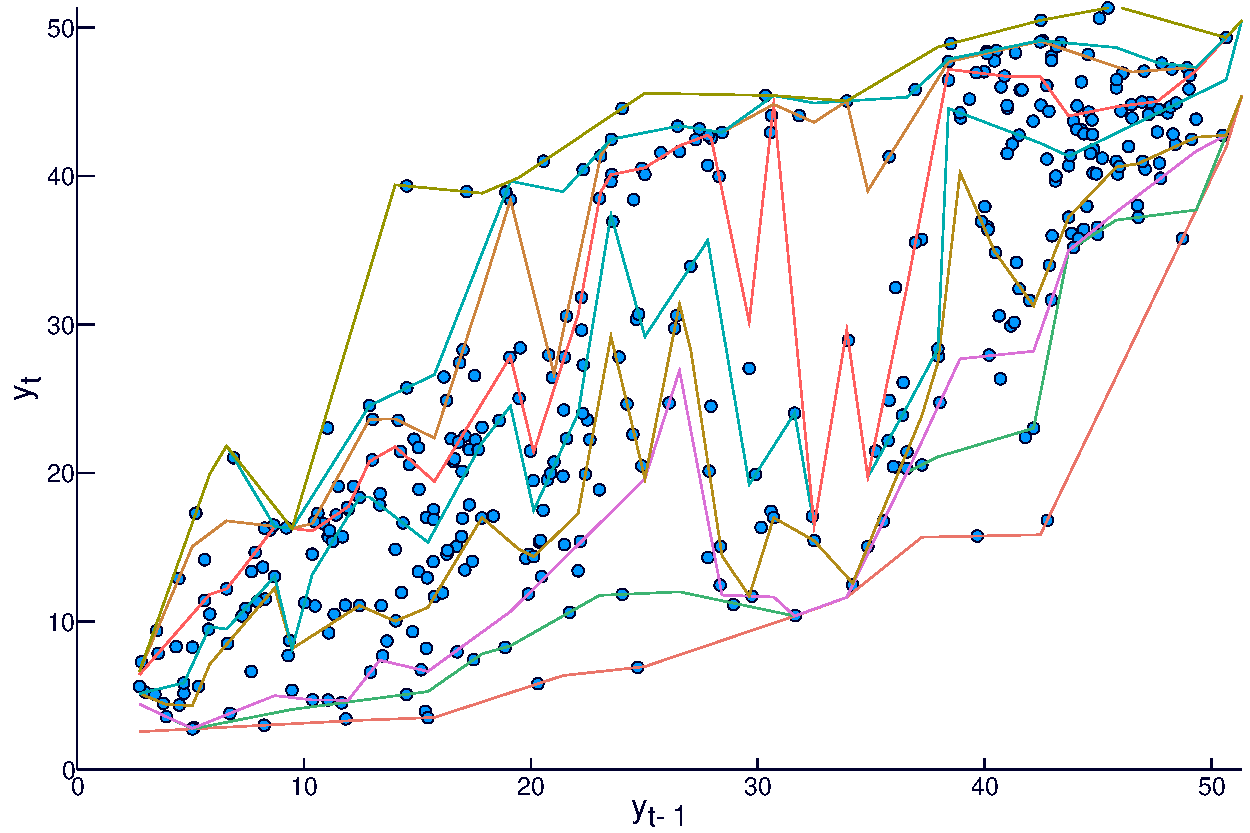
\includegraphics[width=\textwidth]{Figuras/regressao-quantilica/icaraizinho-crossing-01}
      \subcaption{$\lambda_1 = 0, \, \lambda_2 = 0.1$}
    \end{minipage}
    \begin{minipage}[b]{\linewidth}
      \centering     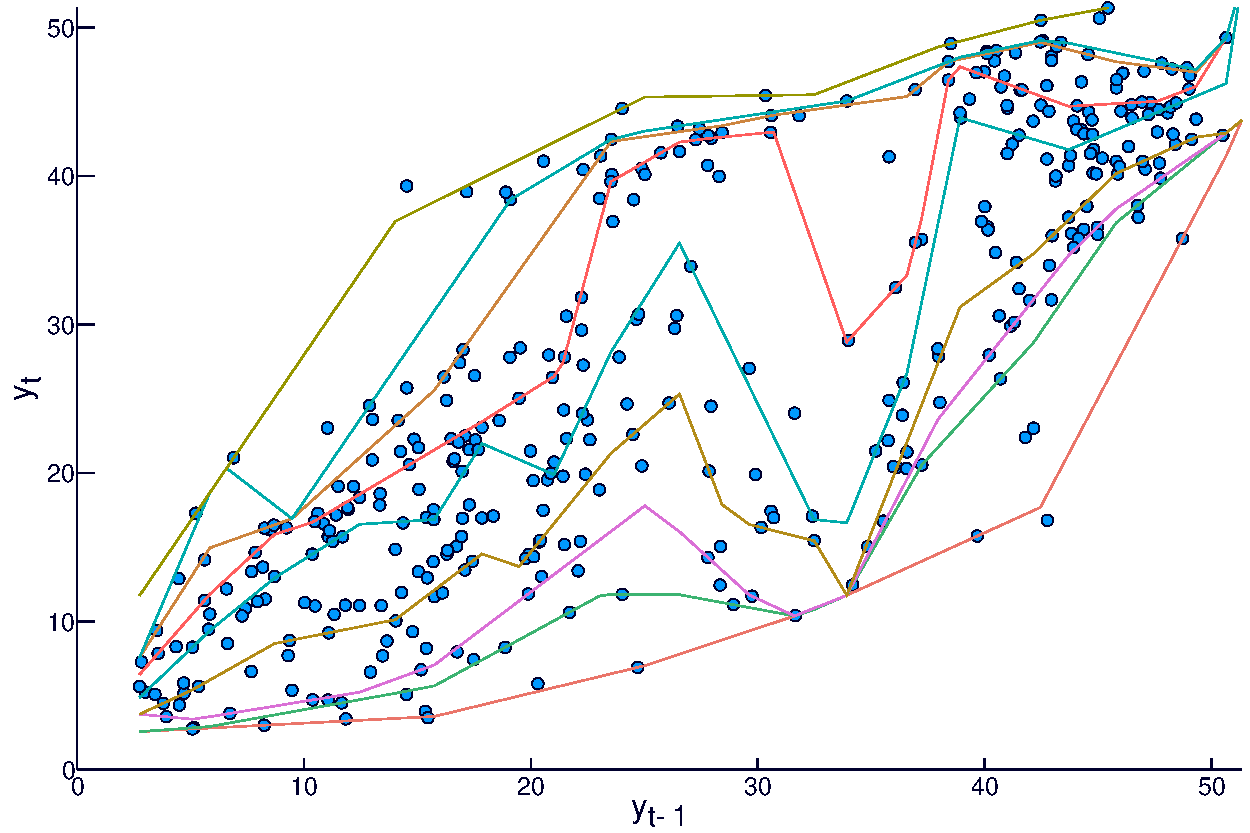
\includegraphics[width=\textwidth]{Figuras/regressao-quantilica/icaraizinho-crossing-03}
      \subcaption{$\lambda_1 = 0, \, \lambda_2 = 0.3$}
    \end{minipage}
     \begin{minipage}[b]{\linewidth}
      \centering     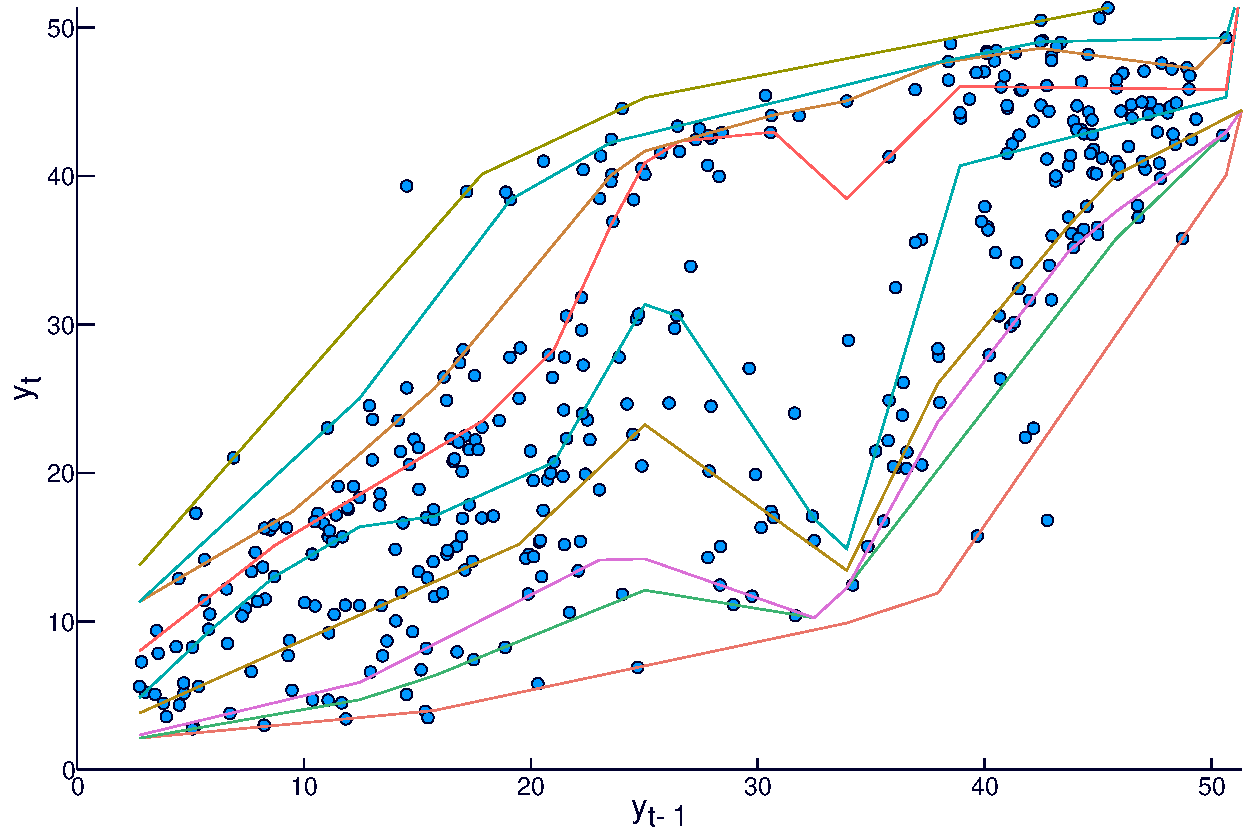
\includegraphics[width=\textwidth]{Figuras/regressao-quantilica/icaraizinho-crossing-1}
      \subcaption{$\lambda_1 = 0, \, \lambda_2 = 1$}
     \end{minipage}
  \end{minipage}
  \begin{minipage}[t]{0.4\linewidth}
    \centering
    \begin{minipage}[t]{\linewidth}
      \centering     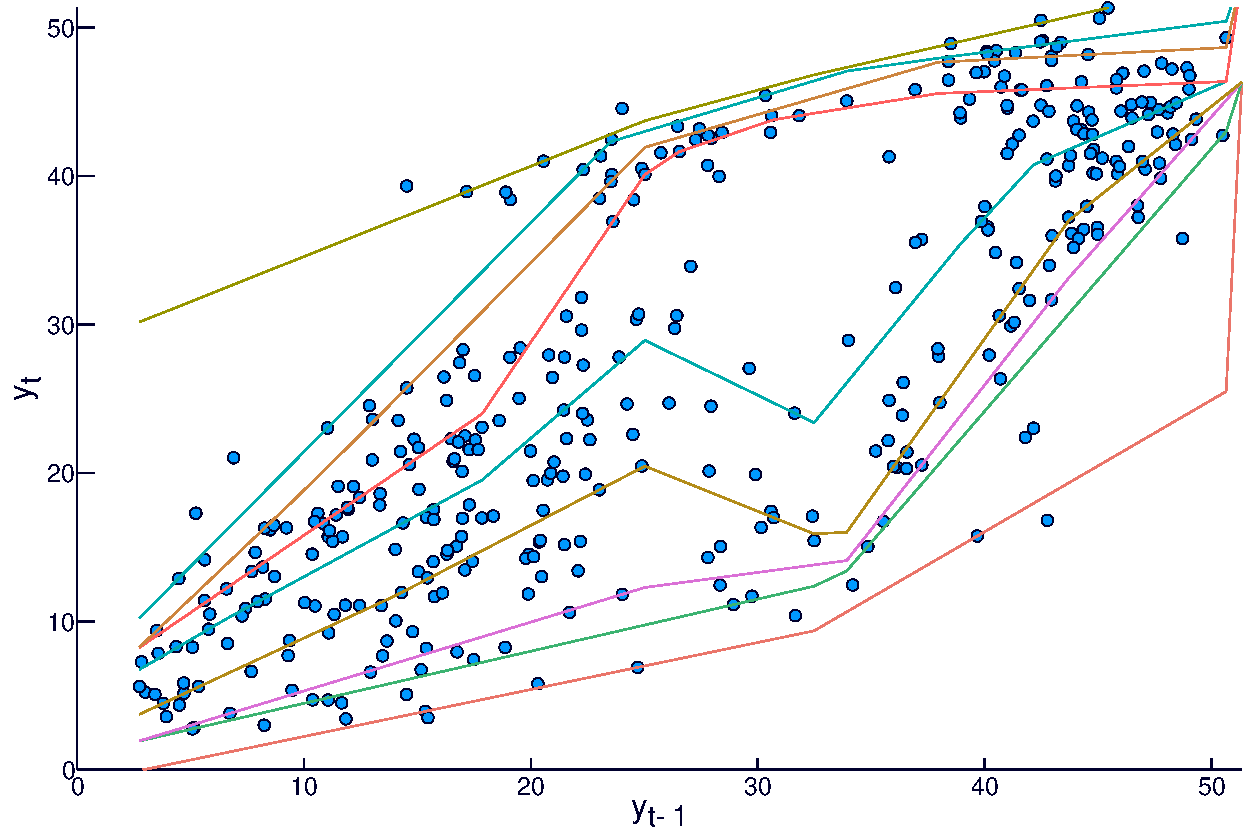
\includegraphics[width=\textwidth]{Figuras/regressao-quantilica/icaraizinho-crossing-3}
      \subcaption{$\lambda_1 = 0, \, \lambda_2 = 3$}
    \end{minipage}
    \begin{minipage}[b]{\linewidth}
      \centering     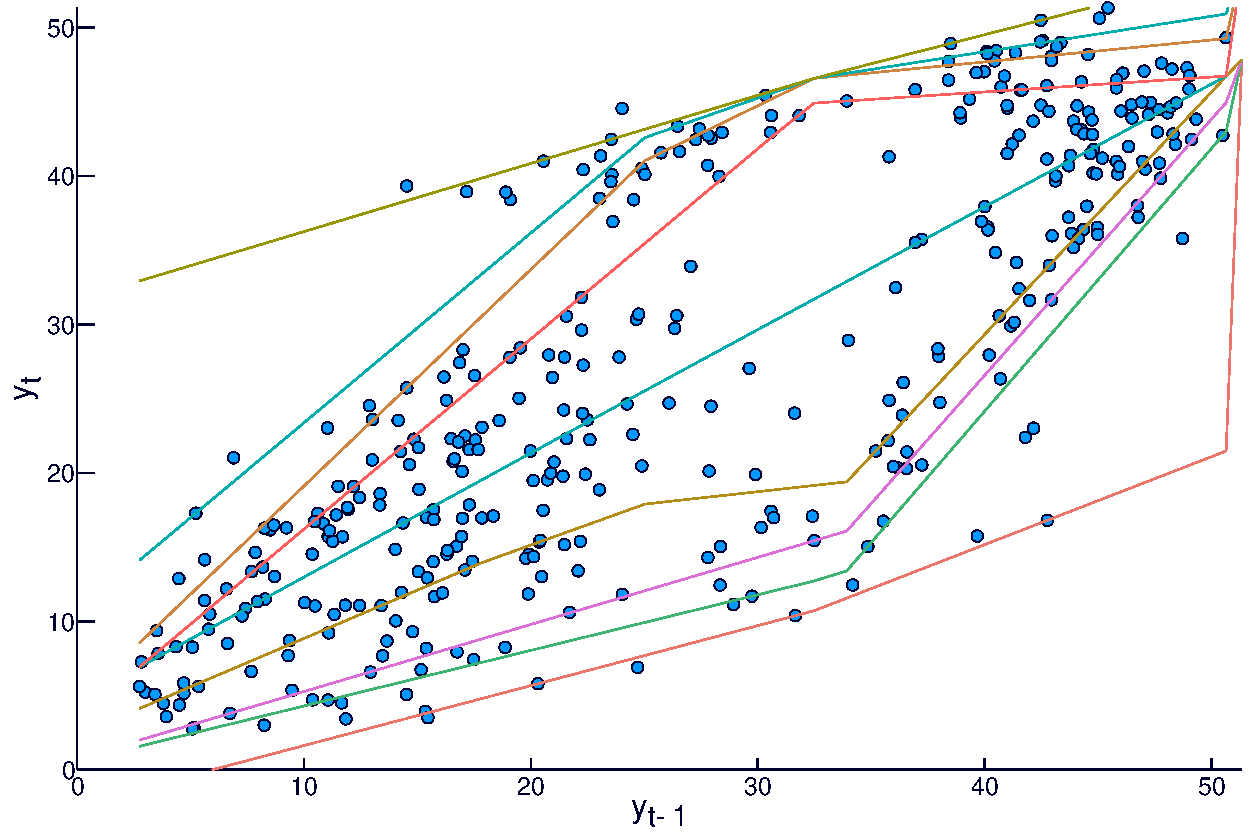
\includegraphics[width=\textwidth]{Figuras/regressao-quantilica/icaraizinho-crossing-10}
      \subcaption{$\lambda_1 = 0, \, \lambda_2 = 10$}
    \end{minipage}
     \begin{minipage}[b]{\linewidth}
      \centering     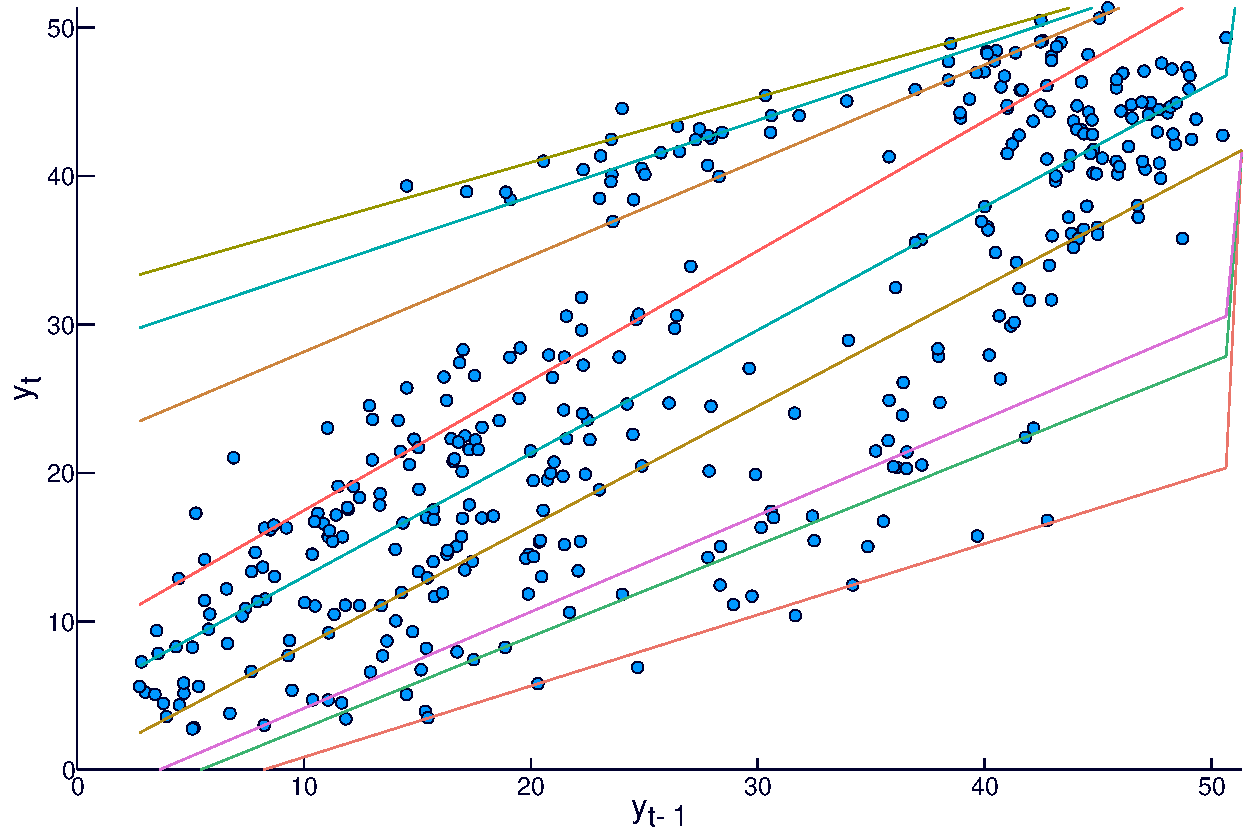
\includegraphics[width=\textwidth]{Figuras/regressao-quantilica/icaraizinho-crossing-200}
      \subcaption{$\lambda_1 = 0, \, \lambda_2 = 200$}
      \label{fig:npqar-cross}
     \end{minipage}
  \end{minipage}
  \caption{Quantile estimations for a few different values of $\lambda_2$. The quantiles represented here are $\alpha = (5\%, 10\%, 25\%, 50\%, 75\%, 90\%, 95\%)$. When $\lambda_2 = 0.1$, on the upper left, we see a overfitting on the estimations. The other extreme case is also shown, when $\lambda_2=200$ the nonparametric estimator converges to the linear model.}
  \label{fig:npqar-results}
\end{figure}

The first issue is how to select an appropriate value for $\lambda_2$. A simple way is to do it by inspection, which means to test many different values and pick the one that suits best our needs by looking at them. The other alternative is to use a metric to which we can select the best tune. We can achieve this by using a cross-validation method, for example.

The other issue occurs when we try to add more than one lag to the analysis at the same time. This happens because the problem solution is a set of points that we need to interpolate. This multivariate interpolation, however, is not easily solved, in the sense that we can either choose using a very naive estimator such as the K-nearest neighbors or just find another method that is not yet adopted for a wide range of applications.

%\subsection{Solar power data}
%
%While the Icaraizinho dataset has monthly observations for a wide range of time, we also test the same model for hourly data. In this case, we use the NP-QAR for solar power data. This dataset was retrieved from \textit{https://www.renewables.ninja/} and includes predicted hourly power data for the city of Tubarão (Brazil).
%This location was chosen because it is the spot of the biggest solar power plant in Brazil. 
%
%
%%Tabocas do Brejo Velho (usina solar "Horizonte" em construção, será a maior da america latina; -12.692, -44.006)
%
%
%%São José de Mipibu (usina solar  http://oportaln10.com.br/grupo-chines-instalara-fabrica-de-placas-solares-no-rn-50324/, -6.068 , -35.241)
%
%% Tubarão -28.467_-49.005_
%
%As solar power production is irradiation dependent, the best single predictor we may have is the hour of the day, as can be seen in the boxplot shown in Figure \ref{fig:solar-tubarao}
%
%\begin{figure}[h]
%	\centering
%	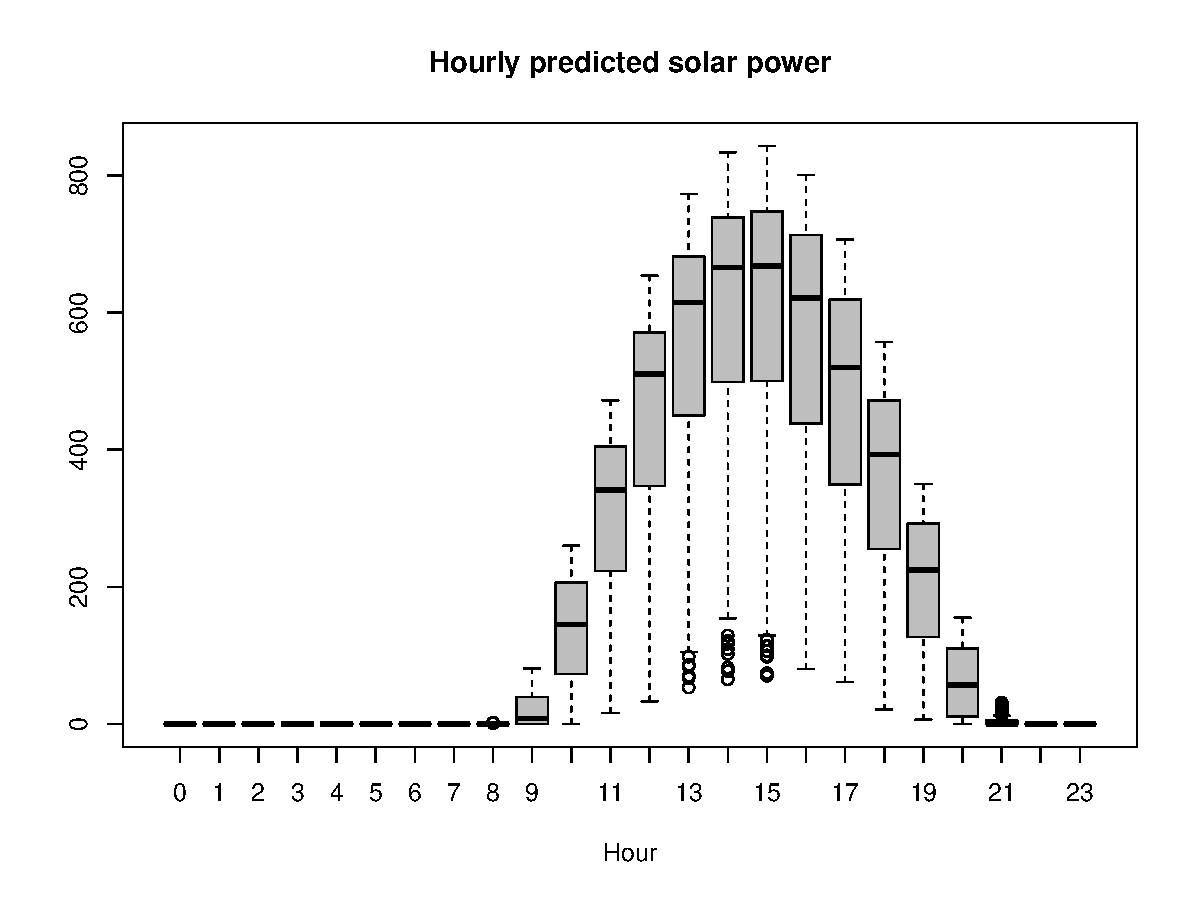
\includegraphics[width=0.8\linewidth]{Figuras/npqar-solar/hourly-solar-power.pdf}
%	\caption{Icaraizinho yearly data. Each serie consists of monthly observations for each year.}
%	\label{fig:solar-tubarao}
%\end{figure}
%
%
%
%
%
%\begin{figure}[h]
%	\centering
%		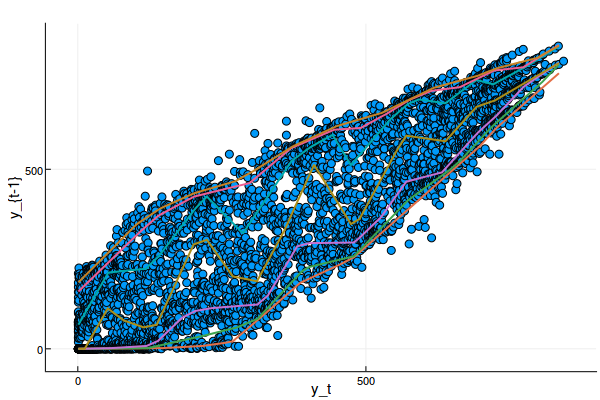
\includegraphics[width=0.8\linewidth]{Figuras/npqar-solar/com-divisao-lambda100.png}
%	\caption{Icaraizinho yearly data. Each serie consists of monthly observations for each year.}
%	\label{fig:npqar-solar-tubarao}
%\end{figure}
